% \appendix

% \part*{Anexos}


% \chapter*{Anexo A: Diagramas UML}
% \renewcommand{\thefigure}{A.\arabic{figure}}
%
% \begin{figure}[ht]
%  \centering
%  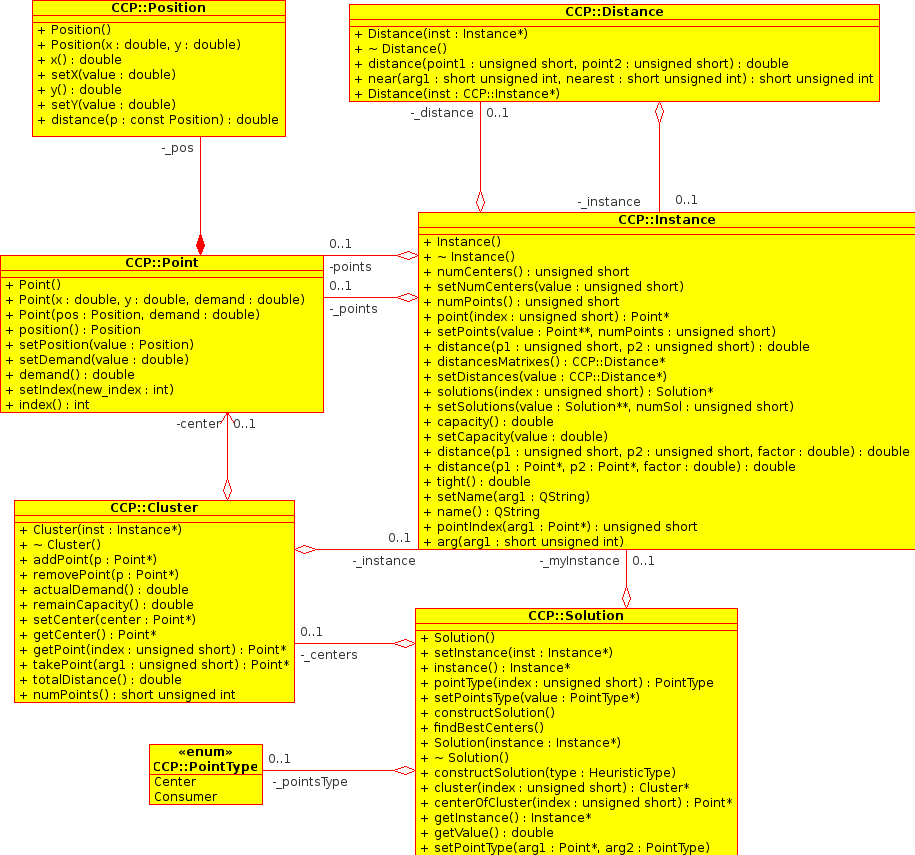
\includegraphics[bb=0 0 794 742,scale=0.4]{../TCC-I/imagens/Instance.png}
%  % Instance.png: 915x855 pixel, 83dpi, 28.00x26.16 cm, bb=0 0 794 742
% \caption{Classes que representam uma Inst�ncia e as solu��es }
% \end{figure}
%
% %
% % \begin{figure}
% %  \begin{center}
% %  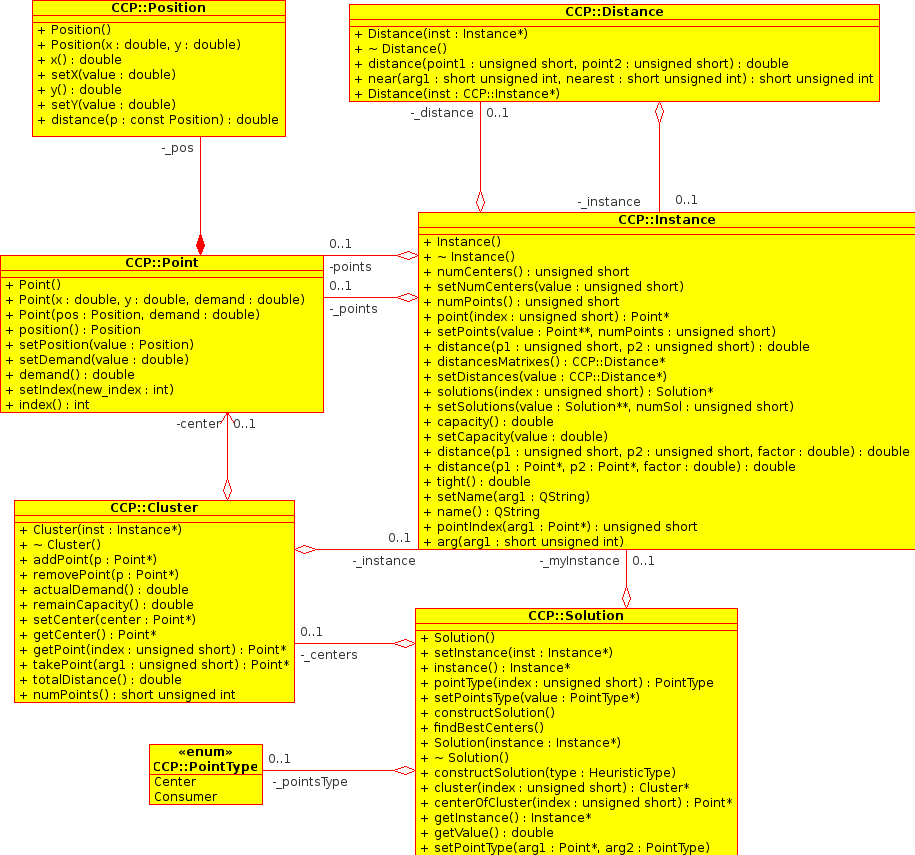
\includegraphics[scale=0.4]{../TCC-I/imagens/Instance.png}
% %  % Instance.png: 915x855 pixel, 83dpi, 28.00x26.16 cm, bb=0 0 794 742
% %
% % \end{center}
% % \end{figure}
%
%
% \begin{figure}[ht]
%  \centering
%  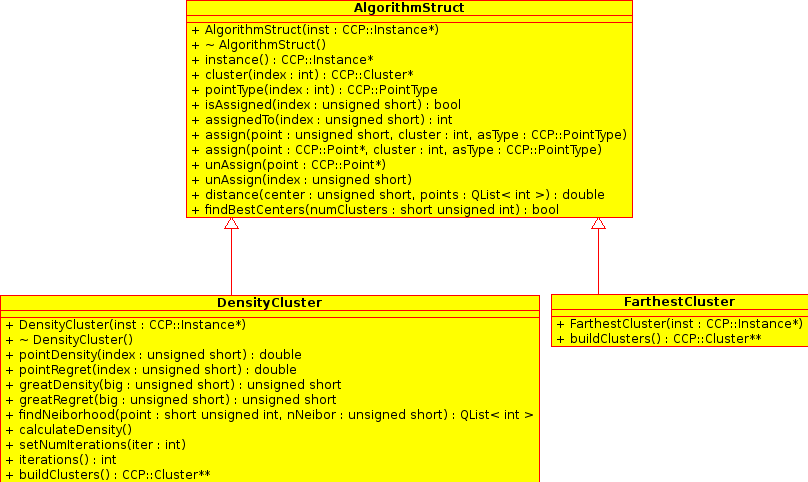
\includegraphics[bb=0 0 701 418, scale=0.6]{../TCC-I/imagens/Algorthms.png}
%  % Algorthms.png: 808x482 pixel, 83dpi, 24.72x14.75 cm, bb=0 0 701 418
% \caption{Classes dos algoritmos das heur�sticas de constru��o}
%
% \end{figure}
% %
% % \begin{figure}
% % \begin{center}
% % 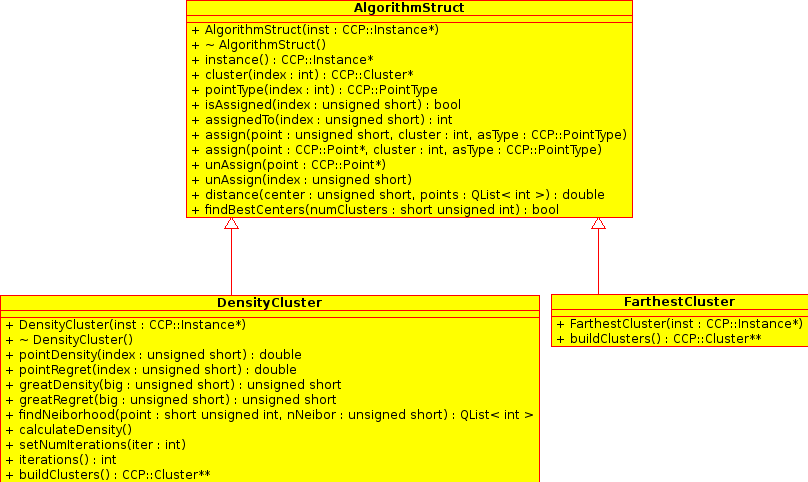
\includegraphics[scale=0.5]{../TCC-I/imagens/Algorthms.png}
% %
% % \end{center}
% % \end{figure}
%
%
% % \begin{landscape}
%
%
% \chapter*{Anexo B: Associa��o dos M�dulos}
% \renewcommand{\thefigure}{B.\arabic{figure}}
% %
% % 
\tikzset{
  arrow/.style={-stealth', line width=0.5pt},
  every picture/.append style={line width=1pt},
}

\tiny {

\enlargethispage{100cm}
% Start of code
% \begin{tikzpicture}[anchor=mid,>=latex',join=bevel,]
\begin{tikzpicture}[>=latex',join=bevel,scale=0.65]
  \pgfsetlinewidth{1bp}
%%
\pgfsetcolor{black}
  % Edge: node0 -> node4
  \draw [->] (130.06bp,219.43bp) .. controls (125.48bp,210.75bp) and (119.51bp,199.45bp)  .. (109.32bp,180.13bp);
  % Edge: node9 -> node12
  \draw [->] (716.02bp,147.39bp) .. controls (712.23bp,146.19bp) and (708.43bp,145.04bp)  .. (704.75bp,144bp) .. controls (632.92bp,123.76bp) and (612.69bp,127.83bp)  .. (540.75bp,108bp) .. controls (537.36bp,107.07bp) and (533.87bp,106.04bp)  .. (520.57bp,101.88bp);
  % Edge: node0 -> node11
  \draw [->] (108.83bp,226.23bp) .. controls (86.415bp,218.52bp) and (56.87bp,204.27bp)  .. (42.75bp,180bp) .. controls (31.694bp,161bp) and (36.774bp,136.1bp)  .. (47.572bp,107.83bp);
  % Edge: node6 -> node1
  \draw [->] (392.12bp,147.43bp) .. controls (390.6bp,139.01bp) and (388.64bp,128.14bp)  .. (385.02bp,108.13bp);
  % Edge: node9 -> node3
  \draw [->] (730.64bp,147.43bp) .. controls (710.16bp,136bp) and (681.55bp,120.03bp)  .. (650.79bp,102.86bp);
  % Edge: node8 -> node2
  \draw [->] (661.03bp,147.43bp) .. controls (677.35bp,137.64bp) and (699.21bp,124.52bp)  .. (726.54bp,108.13bp);
  % Edge: node5 -> node1
  \draw [->] (288.43bp,147.43bp) .. controls (304.26bp,137.68bp) and (325.46bp,124.64bp)  .. (352.29bp,108.13bp);
  % Edge: node2 -> node10
  \draw [->] (723.61bp,74.684bp) .. controls (720.65bp,73.658bp) and (717.67bp,72.741bp)  .. (714.75bp,72bp) .. controls (615.37bp,46.802bp) and (311.96bp,27.968bp)  .. (174.49bp,20.41bp);
  % Edge: node0 -> node1
  \draw [->] (143.2bp,219.19bp) .. controls (151.34bp,199.15bp) and (168.56bp,163.65bp)  .. (194.75bp,144bp) .. controls (234.16bp,114.43bp) and (289.34bp,101.03bp)  .. (339.68bp,93.545bp);
  % Edge: node5 -> node12
  \draw [->] (310.78bp,147.35bp) .. controls (344.57bp,136.56bp) and (391.55bp,121.49bp)  .. (432.75bp,108bp) .. controls (435.9bp,106.97bp) and (439.14bp,105.9bp)  .. (452.2bp,101.58bp);
  % Edge: node9 -> node2
  \draw [->] (756.75bp,147.43bp) .. controls (756.75bp,139.1bp) and (756.75bp,128.37bp)  .. (756.75bp,108.13bp);
  % Edge: node4 -> node1
  \draw [->] (147.76bp,147.85bp) .. controls (152.48bp,146.52bp) and (157.2bp,145.22bp)  .. (161.75bp,144bp) .. controls (218.97bp,128.68bp) and (285.01bp,112.7bp)  .. (339.44bp,99.83bp);
  % Edge: node8 -> node3
  \draw [->] (634.93bp,147.43bp) .. controls (633.86bp,138.89bp) and (632.48bp,127.82bp)  .. (629.95bp,107.6bp);
  % Edge: node6 -> node12
  \draw [->] (413.37bp,147.43bp) .. controls (426.18bp,137.4bp) and (443.46bp,123.88bp)  .. (466.24bp,106.05bp);
  % Edge: node7 -> node3
  \draw [->] (535.22bp,147.43bp) .. controls (553.25bp,136.24bp) and (578.27bp,120.71bp)  .. (606.27bp,103.33bp);
  % Edge: node6 -> node3
  \draw [->] (441.9bp,147.43bp) .. controls (483.67bp,134.52bp) and (544.13bp,115.84bp)  .. (594.23bp,100.36bp);
  % Edge: node4 -> node10
  \draw [->] (103.3bp,143.76bp) .. controls (108.09bp,119.09bp) and (116.69bp,74.86bp)  .. (124.23bp,36.09bp);
  % Edge: node0 -> node2
  \draw [->] (166.67bp,232.82bp) .. controls (294.44bp,227.45bp) and (803bp,204.6bp)  .. (825.75bp,180bp) .. controls (845.2bp,158.96bp) and (820.23bp,132.75bp)  .. (786.59bp,108.02bp);
  % Edge: node5 -> node3
  \draw [->] (320.06bp,147.35bp) .. controls (325.01bp,146.17bp) and (329.97bp,145.03bp)  .. (334.75bp,144bp) .. controls (425.61bp,124.41bp) and (449.45bp,125.42bp)  .. (540.75bp,108bp) .. controls (552.59bp,105.74bp) and (565.3bp,103.19bp)  .. (587.08bp,98.686bp);
  % Edge: node9 -> node1
  \draw [->] (717.25bp,147.4bp) .. controls (713.06bp,146.14bp) and (708.84bp,144.97bp)  .. (704.75bp,144bp) .. controls (589.21bp,116.65bp) and (553.22bp,135.4bp)  .. (423.85bp,105.62bp);
  % Edge: node7 -> node2
  \draw [->] (557.1bp,147.39bp) .. controls (561.03bp,146.21bp) and (564.95bp,145.07bp)  .. (568.75bp,144bp) .. controls (630.08bp,126.78bp) and (649.56bp,128.97bp)  .. (723.47bp,104.84bp);
  % Edge: node7 -> node12
  \draw [->] (506.69bp,147.43bp) .. controls (503.72bp,138.86bp) and (499.86bp,127.75bp)  .. (492.95bp,107.86bp);
  % Edge: node4 -> node11
  \draw [->] (88.899bp,143.83bp) .. controls (83.973bp,135.58bp) and (78.049bp,125.66bp)  .. (67.448bp,107.91bp);
  % Edge: node0 -> node3
  \draw [->] (166.8bp,232.75bp) .. controls (292.79bp,227.2bp) and (786.63bp,203.97bp)  .. (808.75bp,180bp) .. controls (819.6bp,168.24bp) and (818.31bp,156.83bp)  .. (808.75bp,144bp) .. controls (800.64bp,133.12bp) and (727.4bp,113.75bp)  .. (666.77bp,99.032bp);
  % Edge: node8 -> node1
  \draw [->] (581.63bp,147.41bp) .. controls (530.71bp,133.94bp) and (459.89bp,115.19bp)  .. (423.96bp,105.19bp);
  % Edge: node8 -> node12
  \draw [->] (606.39bp,147.43bp) .. controls (582.94bp,136.17bp) and (550.32bp,120.52bp)  .. (515.79bp,103.94bp);
  % Edge: node0 -> node10
  \draw [->] (108.77bp,225.48bp) .. controls (85.409bp,217.26bp) and (53.194bp,202.69bp)  .. (32.75bp,180bp) .. controls (9.7676bp,154.49bp) and (11.08bp,141.75bp)  .. (4.7496bp,108bp) .. controls (1.7995bp,92.274bp) and (-3.9994bp,85.396bp)  .. (4.7496bp,72bp) .. controls (20.241bp,48.28bp) and (48.728bp,34.912bp)  .. (84.051bp,24.816bp);
  % Edge: node7 -> node1
  \draw [->] (485.44bp,147.43bp) .. controls (467.6bp,137.55bp) and (443.66bp,124.29bp)  .. (414.48bp,108.13bp);
  % Node: node11
\begin{scope}
  \definecolor{strokecol}{rgb}{0.0,0.0,0.0};
  \pgfsetstrokecolor{strokecol}
  \draw (57bp,90bp) ellipse (43bp and 18bp);
  \draw (56.75bp,90bp) node {libQtGui.so};
\end{scope}
  % Node: node10
\begin{scope}
  \definecolor{strokecol}{rgb}{0.0,0.0,0.0};
  \pgfsetstrokecolor{strokecol}
  \draw (128bp,18bp) ellipse (47bp and 18bp);
  \draw (127.75bp,18bp) node {libQtCore.so};
\end{scope}
  % Node: node12
\begin{scope}
  \definecolor{strokecol}{rgb}{0.0,0.0,0.0};
  \pgfsetstrokecolor{strokecol}
  \draw (487bp,90bp) ellipse (45bp and 18bp);
  \draw (486.75bp,90bp) node {libQtTest.so};
\end{scope}
  % Node: node9
\begin{scope}
  \definecolor{strokecol}{rgb}{0.0,0.0,0.0};
  \pgfsetstrokecolor{strokecol}
  \draw (800bp,168bp) -- (757bp,180bp) -- (714bp,168bp) -- (714bp,147bp) -- (800bp,147bp) -- cycle;
  \draw (756.75bp,162bp) node {CCPTest};
\end{scope}
  % Node: node8
\begin{scope}
  \definecolor{strokecol}{rgb}{0.0,0.0,0.0};
  \pgfsetstrokecolor{strokecol}
  \draw (696bp,168bp) -- (637bp,180bp) -- (578bp,168bp) -- (578bp,147bp) -- (696bp,147bp) -- cycle;
  \draw (636.75bp,162bp) node {CCPSolution};
\end{scope}
  % Node: node1
\begin{scope}
  \definecolor{strokecol}{rgb}{0.0,0.0,0.0};
  \pgfsetstrokecolor{strokecol}
  \draw (424bp,108bp) -- (340bp,108bp) -- (340bp,72bp) -- (424bp,72bp) -- cycle;
  \draw (381.75bp,90bp) node {CCPModelLib};
\end{scope}
  % Node: node0
\begin{scope}
  \definecolor{strokecol}{rgb}{0.0,0.0,0.0};
  \pgfsetstrokecolor{strokecol}
  \draw (167bp,240bp) -- (138bp,252bp) -- (109bp,240bp) -- (109bp,219bp) -- (167bp,219bp) -- cycle;
  \draw (137.75bp,234bp) node {CCP};
\end{scope}
  % Node: node3
\begin{scope}
  \definecolor{strokecol}{rgb}{0.0,0.0,0.0};
  \pgfsetstrokecolor{strokecol}
  \draw (628bp,108bp) -- (550bp,90bp) -- (628bp,72bp) -- (706bp,90bp) -- cycle;
  \draw (627.75bp,90bp) node {CCPAlgorithms};
\end{scope}
  % Node: node2
\begin{scope}
  \definecolor{strokecol}{rgb}{0.0,0.0,0.0};
  \pgfsetstrokecolor{strokecol}
  \draw (790bp,108bp) -- (724bp,108bp) -- (724bp,72bp) -- (790bp,72bp) -- cycle;
  \draw (756.75bp,90bp) node {CCPIOLib};
\end{scope}
  % Node: node5
\begin{scope}
  \definecolor{strokecol}{rgb}{0.0,0.0,0.0};
  \pgfsetstrokecolor{strokecol}
  \draw (326bp,168bp) -- (265bp,180bp) -- (204bp,168bp) -- (204bp,147bp) -- (326bp,147bp) -- cycle;
  \draw (264.75bp,162bp) node {CCPDistance};
\end{scope}
  % Node: node4
\begin{scope}
  \definecolor{strokecol}{rgb}{0.0,0.0,0.0};
  \pgfsetstrokecolor{strokecol}
  \draw (148bp,180bp) -- (52bp,180bp) -- (52bp,144bp) -- (148bp,144bp) -- cycle;
  \draw (99.75bp,162bp) node {CCPClusterView};
\end{scope}
  % Node: node7
\begin{scope}
  \definecolor{strokecol}{rgb}{0.0,0.0,0.0};
  \pgfsetstrokecolor{strokecol}
  \draw (560bp,168bp) -- (512bp,180bp) -- (464bp,168bp) -- (464bp,147bp) -- (560bp,147bp) -- cycle;
  \draw (511.75bp,162bp) node {CCPRead};
\end{scope}
  % Node: node6
\begin{scope}
  \definecolor{strokecol}{rgb}{0.0,0.0,0.0};
  \pgfsetstrokecolor{strokecol}
  \draw (446bp,168bp) -- (395bp,180bp) -- (344bp,168bp) -- (344bp,147bp) -- (446bp,147bp) -- cycle;
  \draw (394.75bp,162bp) node {CCPModel};
\end{scope}
%
\end{tikzpicture}
% End of code

}
% \begin{figure}[ht]
%  \centering
%  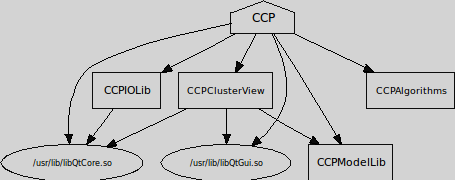
\includegraphics[bb=0 0 341 135]{./images/Modules.png}
%  % Modules.png: 455x180 pixel, 96dpi, 12.04x4.76 cm, bb=0 0 341 135
%
% \caption{Bibliotecas que fazem parte do sistema.}
%
% \end{figure}


% \end{landscape}